\section{Portierung von OpenPearl auf den Stm32f7}
Um OpenPEARL auf dem Stm32f7 benutzen zu können musste es davor angepasst werden.\\
Für den Microcontroller Lpc1768 wurde bereits ein Portierung gemacht.\\
Diese konnte als Beispielportierung genutzt werden, auch wenn es natürlich Unterschiede zwischen den Microcontrollern gibt, die beachtet werden mussten.\\
Der Lpc1768 beitzt zum Beispiel einen ARM Cortex-M3 und der Stm32f7 einen ARM Cortex-M7.\\
Zudem verfügt der Stm32f7 über ein Farbdisplay welches in unserer Anwendung gut hätte eingesetzt werden können.\\
\\
Um herauszufinden ob OpenPEARL auf dem Stm32f7 läuft, sollte ein Testprogramm in pearl geschrieben werden welches eine LED des Microcontrollers blinken lässt.\\
Doch davor musste OpenPEARL für den Stm32f7 portiert werden.\\
Das von komplette uns \nameref{abgeänderte OpenPearl-Projekt} befindet sich in unserem Repository.\\
Im OpnePearl-Projekt gibt es einen Ordner runtime.\\
In ihm sind unter anderem die Portierungsdateien für Linux und Lpc1768.\\
Für unsere Portierung wurde also der Ordner lpc1768 kopiert, in stm32f7 umbenannt und an unser Zielsystem angepasst.\\
\\
Damit der Ordner stm32f7 bei einem "make install" bearbeitet wird, muss zunächst die Makefile im Ordner runtime angepasst werden, sodass stm32f7 als Target hinzugefügt wird.\\
Die folgende Abbildung zeigt ein Beispiel dieser Änderung.\\
Die komplette \nameref{Änderungen der Makefile im Ordner runtime} befinden sich im Anhang.\\
\begin{figure}[h]
\begin{center}
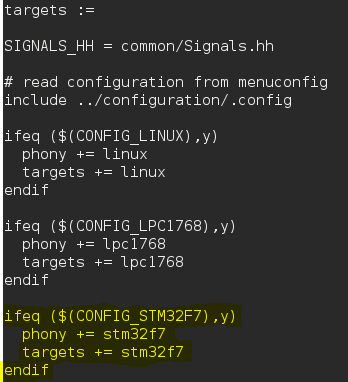
\includegraphics[width=8cm]{grafiken/Makefile_runtime1.png}
\caption{Makefile im Ordner runtime}
\label{Makefile_runtime}
\end{center}
\end{figure}
\newpage
\noindent
Die im Text gelb markierten Stellen wurden neu in die Makefile eingefügt.\\
Mit diesen Änderungen wurde von nun an der Ordner stm32f7 im Ordner runtime bei einem "make" im Oberverzeichnis berücksichtigt.\\
\\
Nun musste im Ordner smt32f7 alles was mit dem Lpc1768 zu tun hatte entweder rausgeschmissen, oder ersetzt werden.\\
Zum Beispiel musste die Makefile, die für den Lpc1768 gemacht wurde, auf den Stm32f7 abgestimmt werden.\\
Dabei wurde wieder das gleiche Vorgehen wie in der Makefile eine Ordnerstruktur höher angewandt.\\
Entweder Alles was mit Lpc1768 zu tun hat auskommentieren, oder stm32f7 spezifisch ersetzen.\\
In der Makefile wurde ein Includepfad(../cortexM/stm32f7HAL/Inc) für den stm32f7 eingefügt.\\
Als Include wurde die HAL-library eingesetzt, in der unter anderem ein Treiber für den I2C des stm32f7 enthalten ist.\\ 
Die folgende Abbildung zeigt einen Teil Änderungen der Makefile im Ordner stm32f7. Die Komplette \nameref{Änderungen der Makefile im Ordner stm32f7} befinden sich im Anhang.\newpage
\begin{figure}[h]
\begin{center}
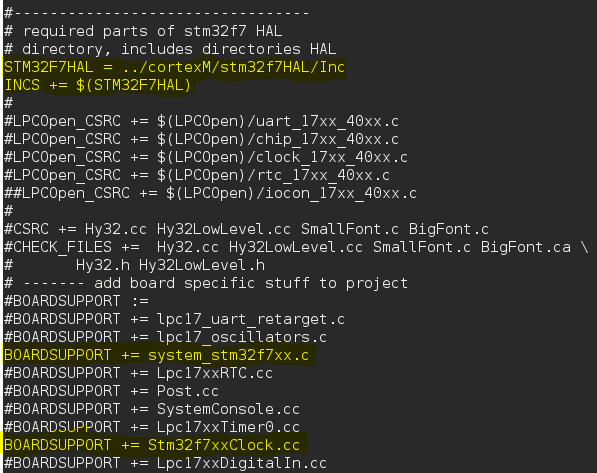
\includegraphics[width=13cm]{grafiken/Makefile_stm32f7_1.png}
\caption{Makefile im Ordner stm32f7}
\label{Makefile_stm32f7}
\end{center}
\end{figure}
\noindent
Des Weiteren wurden die Dateien {\textit{system\_stm32f7xx.c}}, {\textit{Stm32f7xxClock.cc}} und {\textit{startup\_stm32f4xx.S}} als Boardsupport angegeben.\\
Diese Dateien mussten natürlich vorhanden oder neu erstellt werden.\\
Die {\textit{startup\_stm32f4xx.S}} ist eine Vorbereitung für den Microcontroller, die vor dem Laufen eines Programms durchgeführt wird.\\ 
Die {\textit{system\_stm32f7xx.c}} ist für Registerdeclerationen, Bitdeclerationen und Macros da, um auf Register der Hardware zugreifen zu können.\\
\\
\newpage
\noindent
Im Ordner "tests" befinden sich Test- und Beispielprogramme.\\
Die Datei Makefile.inc beschreibt, welche Testprogramme bei einem Makebefehl durchgeführt werden.\\
In der Makefile.inc wurden alle Tests des Lpc1768 herausgenommen und ein neuer Test für unser Blinkprogramm(digitaliotest.cc) eingetragen.\\
\begin{figure}[h]
\begin{center}
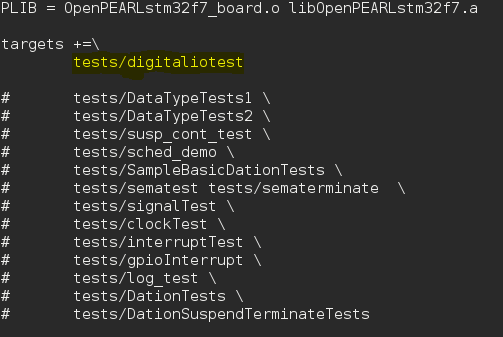
\includegraphics[width=12cm]{grafiken/Makefile_tests.png}
\caption{Makefile im Ordner tests}
\label{Makefile_tests}
\end{center}
\end{figure}
\\
Die mit Raute markierten Zeilen sind Kommentare.\\
Der Name digitaliotest.cc kommt daher, dass es diesen Test schon beim Lpc1768 gab und Teile des Programms für die Blinkyanwendung übernommen wurden.\\
\\
Bei einem make-install-Befehl im obersten Verzeichnis wird nun unter anderem die Datei Pearlincludes.h erstellt und das Programm digitaliotest durchgeführt.\\
Um nicht jedes Mal aufs neue einen Makebefehl durchführen zu müssen, wurde das prl-Skript angepasst.\\ 
Der stm32f7 wurde als neues "target" eingefügt.\\
Nun konnte ganz leicht mit dem Befehl {\textit{prl -b stm32f7 digitaliotest.cc}} aus der C++-Datei eine ausführbare Datei generiert werden.\\
Mit dem Befehl {\textit{objcopy -O binary -I elf32-little digitaliotest test.bin}} wurde die Datei digitaliotest.elf in die Datei test.bin(Binärdatei) umgewandelt.\\
Zuletzt wurde die Datei test.bin mit dem Befehl {\textit{st-flash write test.bin 0x8000000}} auf das Board geladen.\\
\\
Doch anders als im Programm vorgesehen, blinkte die angesteuerte LED nicht.\\
Hierfür kann es viele Gründe geben.\\
Es kann sein das FreeRTOS nicht richtig auf dem Microcontroller läuft oder ein anderer Aspekt bei der Portierung übersehen wurde.\\
Da auch der Debugger nicht richtig funktionierte war es schwierig genaueres in Erfahrung zu bringen.\\

